\vspace{10pt}
\subsubsection*{\bf Data Analysis}
\vspace{3pt}
\noindent {\sf [Spokesperson :\ Hideyuki Tagoshi]}

\vspace{3pt}
\noindent {\sf \small ICRR, The Univ.\ of Tokyo, Kashiwa, Chiba, 277-8582}

\vspace{3pt}
There are variety of data related activities in KAGRA. 
The main data server of KAGRA is located at ICRR Kashiwa. It has a 2.5PiB data storage. 
All KAGRA data taken at Kamioka are packed into one file for every 32 seconds, 
and are transferred continuously to the main data server at Kashiwa. Beside this, low latency data transfer 
is also done by packing only main interferometer data into one file for every 1 seconds. 
For low latency data transfer, the latency of about 3 seconds is achieved from Kamioka to Kashiwa
(this time include the time necessary for calibration). 

KAGRA detector is producing several hundreds thousands of channels of data which record 
signals from various sensors, signals to control instruments, signals to monitor environment of the detector. 
Those data are used to check the status of detector and to improve the sensitivity. 
It is important to introduce convenient tools to visualize the data in order to accelerate the installation 
and commissioning works.  
Web based visualization tools are now being developed. Some of tools developed by LIGO group are also installed. 
These tools are also useful when gravitational wave signals are detected. 
In order to have a confidence of detection of gravitational wave signals, 
it is important to investigate environmental channels whether there are any noise sources which might 
produce data which are similar to real gravitational wave signals. 
These visualization tools can be used to check various  environmental channel data. 


In order to detect gravitational wave signals, several pipelines have been developed in KAGRA. 
Among them, a pipeline to search for gravitational waves from compact binary coalescences (CBC) 
are developed in KAGRA Algorithmic Library (KAGALI). KAGALI is a common data analysis library 
written mainly in C. The CBC pipeline have been used to analyze KAGRA data during iKAGRA operation. 
Improvement of the CBC pipeline are now ongoing in order to treat multiple detectors and 
to introduce the spin parameters in the waveform. These tasks will be continued in 2019. 
The improvement of the parameter estimation pipeline for CBC signals 
based on the Markov Chain Monte Carlo method was continued from the last year. 
This work is lead by Hyung Won Lee (Inje Univ). 

There are several efforts to introduce new data analysis methods in the analysis of gravitational wave data. 
Among them, the performance of Non-Harmonic Analysis (NHA) in visualizing the time-frequency behavior 
of the data was evaluated. NHA is a method to evaluate the spectrum of data 
by evaluating multiple instantaneous frequencies and amplitudes of data in a way which is different from 
discrete Fourier transform. We find that there are various advantage in NHA in visualizing CBC signals 
compared with the method of short time Fourier transform. We apply NHA to public data of 
LIGO-Virgo events, like GW150914, GW170817, and demonstrated the visualization of the signal 
on time-frequency plane. This work has been done in collaboration with the group of Shigeki Hirobayashi
(Univ. Toyama). 

~\\
\noindent
Ref.~~Kenta Yanagisawa , Dongbao Jia, Shigeki Hirobayashi, Nami Uchikata , Tatsuya Narikawa, Koh Ueno, Hirotaka Takahashi, Hideyuki Tagoshi, PTEP 2019 (2019) no.6, 063F01.

\begin{figure} [hbtp]
\begin{center}
%\includegraphics[width=6cm, bb=0 0 1208 909, angle=-90]{astrodiv/gw/das/fig/figdas.pdf}
\includegraphics[width=6cm, angle=-90]{astrodiv/gw/das/fig/figdas.pdf}
%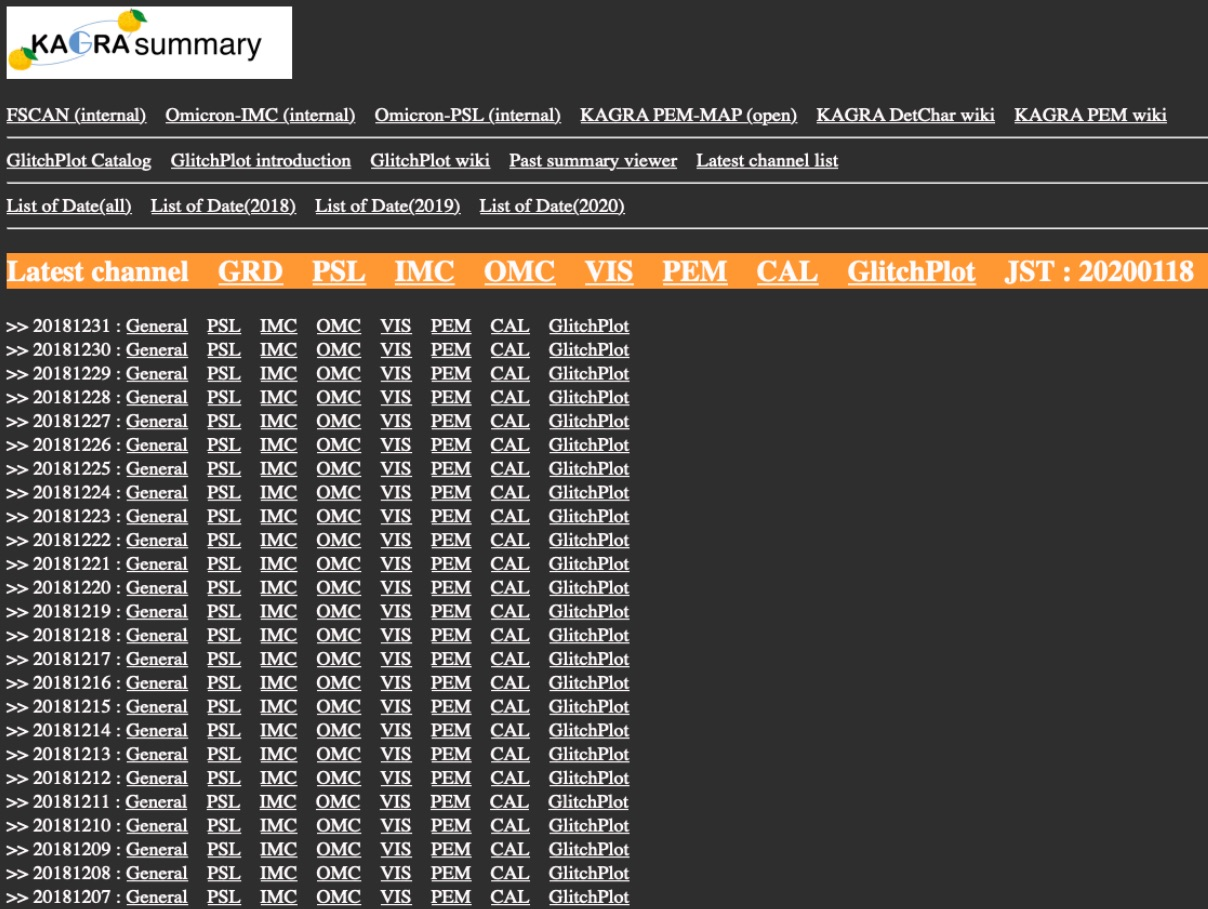
\includegraphics[width=0.4\textwidth, bb=0 0 1208 909]{fig_da.jpg}
%\includegraphics[width=0.4\textwidth]{fig/figdas.pdf}
\caption{\utsm \noindent{\narrower{Example of summary page}}}
\label{fig:KAGRA_DA_Sum}
\end{center}
\end{figure}


